% ------------------------------------------------------------------------------
% TYPO3 CMS 6.2 LTS - What's New - Chapter "In-Depth Changes" (Spanish Version)
%
% @author	Sergio Catalá <sergio.catala@e-net.info>
% @author	Michel Mix <mmix@autistici.org>
% @license	Creative Commons BY-NC-SA 3.0
% @link		http://typo3.org/download/release-notes/whats-new/
% @language	Spanish
% ------------------------------------------------------------------------------
% Chapter: In-Depth Changes
% ------------------------------------------------------------------------------

\section{Cambios en Profundidad}
\begin{frame}[fragile]
	\frametitle{Cambios en Profundidad}

	\begin{center}\huge{Capítulo 6:}\end{center}
	\begin{center}\huge{\color{typo3darkgrey}\textbf{Cambios en Profundidad}}\end{center}

\end{frame}

% ------------------------------------------------------------------------------
% normalize.css
% ------------------------------------------------------------------------------
% http://forge.typo3.org/issues/47920

\begin{frame}[fragile]
	\frametitle{Cambios en Profundidad}
	\framesubtitle{Normalize.css}

	\begin{itemize}
		\item La interfaz de usuario del backend hace uso de \texttt{normalize.css},\newline
			que hace que los navegadores procesen todos los elementos más consistentemente y conforme a los estándares modernos
		\item Alternativa moderna, lista en HTML5, al tradicional reseteado de CSS
		\item Los objetivos de \texttt{normalize.css} son:

			\begin{itemize}
				\item Preservar valores predeterminados útiles del navegador en lugar de borrarlos
				\item Normalizar los estilos de una amplia gama de elementos HTML
				\item Corregir los errores e inconsistencias comunes del navegador
				\item Mejorar la usabilidad con sutiles mejoras
				\item Explicar el código usando comentarios y documentación detallada
			\end{itemize}

	\end{itemize}

\end{frame}

% ------------------------------------------------------------------------------
% displayCond options BIT and !BIT
% ------------------------------------------------------------------------------
% http://forge.typo3.org/issues/45514

\begin{frame}[fragile]
	\frametitle{Cambios en Profundidad}
	\framesubtitle{Opciones BIT y !BIT en TCA: displayCond}

	\lstset{
		basicstyle=\tiny\ttfamily
	}

	\begin{itemize}
		\item Comprobación con un campo de múltiples valores en \texttt{displayCond} (bit a bit)\newline
			\texttt{BIT}: bit está activo, \texttt{!BIT}: bit \underline{no} está activo
	\end{itemize}

	\begin{columns}[T]

		\begin{column}{.5\textwidth}

			\advance\leftskip+1cm
			Suponiendo este TCA:

			\lstset{xleftmargin=1cm}

			\begin{lstlisting}
				'content' => array(
				  'label' => '...',
				  'config' => array(
				    'type' => 'check',
				    'items' => array(
				      array('Contenido A', ''),
				      array('Contenido B', ''),
				      array('Contenido C', ''),
				    ),
				  )
				),
			\end{lstlisting}

		\end{column}
		\begin{column}{.5\textwidth}

			Ejemplos:

			\begin{lstlisting}
				'content_a' => array(
				  'label' => '...',
				  'displayCond' => 'FIELD:content:BIT:1',
				  'config' => array(
				    'type' => 'text',
				  )
				),

				'content_b' => array(
				  'label' => '...',
				  'displayCond' => 'FIELD:content:!BIT:2',
				  'config' => array(
				    'type' => 'text',
				  )
				),
			\end{lstlisting}
		\end{column}

	\end{columns}

\end{frame}

% ------------------------------------------------------------------------------
% Automatic language updates for extensions
% ------------------------------------------------------------------------------
% http://forge.typo3.org/issues/43703

\begin{frame}[fragile]
	\frametitle{Cambios en Profundidad}
	\framesubtitle{Actualizaciones de Idiomas}

	\begin{itemize}
		% \item Extbase Command Controller allows to update translations of extensions for selected languages
		\item Extbase Command Controller permite actualizaciones del idioma para las extensiones:

			\begin{lstlisting}
				$GLOBALS['TYPO3_CONF_VARS']['SC_OPTIONS']['extbase']
				  ['commandControllers'][] =
				  'TYPO3\\CMS\\Lang\\Command\\LanguageCommandController';
			\end{lstlisting}

		\item Llamada de ejemplo:

			\lstinline!typo3/cli_dispatch.phpsh extbase language:update de,en,fr!

		\item Lista separada por comas de configuraciones regionales (p.ej. \texttt{de,en,fr}) limita la actualización de estos idiomas
		\item Sin este argumento, se actualizan todos los idiomas que se encuentran en el módulo "Idiomas"

	\end{itemize}

\end{frame}

% ------------------------------------------------------------------------------
% Migrate system extension manuals to reStructured Text
% ------------------------------------------------------------------------------
% http://forge.typo3.org/issues/50052

\begin{frame}[fragile]
	\frametitle{Cambios en Profundidad}
	\framesubtitle{Extensiones del sistema: Manuales de ReST}

	\begin{itemize}
		\item Todos los manuales de extensiones del sistema se migran a reStructuredText
		\item Manuales de OpenOffice ya no se utilizan y se han eliminado
		\item ReST es un sistema analizador y una sintaxis de marcado de texto plano, fácil de leer, lo que ves es lo que obtienes
		\item Los archivos de ReST de extensiones del sistema se guardan en:\newline
			\texttt{typo3/sysext/<extensionkey>/Documentation/*}

		\item Más información:

			\begin{itemize}
				\item \url{http://es.wikipedia.org/wiki/ReStructuredText}
				\item \url{http://wiki.typo3.org/ReST}
			\end{itemize}

	\end{itemize}

\end{frame}

% ------------------------------------------------------------------------------
% Support custom translation servers for extensions
% ------------------------------------------------------------------------------
% http://forge.typo3.org/issues/50052

\begin{frame}[fragile]
	\frametitle{Cambios en Profundidad}
	\framesubtitle{Servidores Personalizados de Traducciones (1)}

	\begin{itemize}
		\item Se implementó soporte de servidores personalizados de traducciones para las extensiones
		\item Con el uso de XLIFF y una nueva Signal/Slot,\newline
			esto es pan comido (consulte la siguiente diapositiva para ver un ejemplo)
		\item Una posible solución para el servidor de traducción: \textbf{Pootle}

			\begin{itemize}
				\item herramienta de gestión de traducción en línea con una interfaz de traducción
				\item escrito en Python usando Django
				\item originalmente desarrollado y lanzado por \url{translate.org.za}
				\item licencia GNU GPL
			\end{itemize}

	\end{itemize}

\end{frame}

% ------------------------------------------------------------------------------
% Support custom translation servers for extensions
% ------------------------------------------------------------------------------
% http://forge.typo3.org/issues/50052

\begin{frame}[fragile]
	\frametitle{Cambios en Profundidad}
	\framesubtitle{Servidores de Traducciones Personalizados (2)}

	Ejemplo: \texttt{EXT:myextension/localconf.php}

	\lstset{
		basicstyle=\tiny\ttfamily
	}

	\begin{lstlisting}
		/**
		 * @var \TYPO3\CMS\Extbase\SignalSlot\Dispatcher $signalSlotDispatcher
		 */
		$signalSlotDispatcher =
		  \TYPO3\CMS\Core\Utility\GeneralUtility::makeInstance(
		    'TYPO3\\CMS\\Extbase\\SignalSlot\\Dispatcher');

		$signalSlotDispatcher->connect(
		  'TYPO3\\CMS\\Lang\\Service\\UpdateTranslationService',
		  'postProcessMirrorUrl',
		  'Company\\Extension\Slots\\CustomMirror',
		  'postProcessMirrorUrl'
		);
	\end{lstlisting}

\end{frame}

% ------------------------------------------------------------------------------
% Support custom translation servers for extensions
% ------------------------------------------------------------------------------
% http://forge.typo3.org/issues/50052

\begin{frame}[fragile]
	\frametitle{Cambios en Profundidad}
	\framesubtitle{Servidores de Traducciones Personalizados (3)}

	Ejemplo: \texttt{EXT:myextension/Classes/Slots/CustomMirror.php}

	\lstset{
		basicstyle=\tiny\ttfamily
	}

	\begin{lstlisting}
		<?php
		namespace Company\Extensions\Slots;
		class CustomMirror {

		  /**
		   * @var string
		   */
		  protected static $extKey = 'myextension';

		  public function postProcessMirrorUrl($extensionKey, &$mirrorUrl) {
		    if ($extensionKey === self::$extKey) {
		      $mirrorUrl = 'http://example.com/typo3-packages/';
		    }
		  }

		}
	\end{lstlisting}

\end{frame}

% ------------------------------------------------------------------------------
% Support custom translation servers for extensions
% ------------------------------------------------------------------------------
% http://forge.typo3.org/issues/50052

\begin{frame}[fragile]
	\frametitle{Cambios en Profundidad}
	\framesubtitle{Servidores de Traducciones Personalizados (4)}

	Estructura esperada del archivo/directorio en servidor:

	\begin{lstlisting}
		http://example.com/typo3-packages/
		 `-- <first-letter-of-extension-key>
		     `-- <second-letter-of-extension-key>
		         `-- <extension-key>-l10n
		             |-- <extension-key>-l10n-de.zip
		             |-- <extension-key>-l10n-fr.zip
		             |-- <extension-key>-l10n-it.zip
		             `-- <extension-key>-l10n.xml
	\end{lstlisting}

	Por ejemplo:

	\begin{lstlisting}
		http://example.com/typo3-packages/m/y/myextension-l10n/myextension-l10n.xml
	\end{lstlisting}

\end{frame}

% ------------------------------------------------------------------------------
% Support custom translation servers for extensions
% ------------------------------------------------------------------------------
% http://forge.typo3.org/issues/50052

\begin{frame}[fragile]
	\frametitle{Cambios en Profundidad}
	\framesubtitle{Servidores de Traducciones Personalizados (5)}

	Ejemplo: \texttt{<clave-de-extensión>-l10n.xml}

	\lstset{
		basicstyle=\tiny\ttfamily
	}

	\begin{lstlisting}
		<?xml version="1.0" standalone="yes" ?>
		  <TERlanguagePackIndex>
		    <meta>
		      <timestamp>1374841386</timestamp>
		      <date>2013-07-26 14:23:06</date>
		    </meta>
		    <languagePackIndex>
		    <languagepack language="es">
		      <md5>1cc7046c3b624ba1fb1ef565343b84a1</md5>
		    </languagepack>
		    <languagepack language="de">
		     <md5>f00f73ae5c43cb68392e6c508b65de7a</md5>
		    </languagepack>
		    <languagepack language="nl">
		     <md5>cd59530ce1ee0a38e6309544be6bcb3d</md5>
		    </languagepack>
		  </languagePackIndex>
		</TERlanguagePackIndex>
	\end{lstlisting}

\end{frame}

% ------------------------------------------------------------------------------
% Automatic import of t3d files for extensions
% ------------------------------------------------------------------------------
% http://forge.typo3.org/issues/51437

\begin{frame}[fragile]
	\frametitle{Cambios en Profundidad}
	\framesubtitle{Importación Automática de t3d}

	\begin{itemize}
		\item Las extensiones ahora pueden importar \textbf{paquetes t3d} iniciales\newline
			automáticamente durante la instalación de la extensión
		\item Archivos t3d contienen cosas tales como datos, relaciones, archivos, etc..
		\item El archivo t3d tiene que ser llamado \texttt{data.t3d} y situado en:\newline
			\texttt{EXT:myextension/Initialisation/}

		\item La importación ocurre sólo \underline{una vez}\newline
			(incluso si la extensión se instala de nuevo más tarde)

	\end{itemize}

\end{frame}

% ------------------------------------------------------------------------------
% Automatic import of files for extensions
% ------------------------------------------------------------------------------
% http://forge.typo3.org/issues/51446

\begin{frame}[fragile]
	\frametitle{Cambios en Profundidad}
	\framesubtitle{Importación Automática de Archivos}

	\begin{itemize}
		\item Las extensiones ahora pueden importar \textbf{archivos} iniciales\newline
			automáticamente durante la instalación de extensión
		\item Los archivos se copian a:\newline
			\texttt{fileadmin/<extensionkey>/}
		\item Los archivos tienen que situarse en:\newline
			\texttt{EXT:myextension/Initialisation/Files/...}

		\item La importación ocurre \underline{sólo una vez}\newline
			(incluso si la extensión se instala de nuevo más tarde)

	\end{itemize}

\end{frame}

% ------------------------------------------------------------------------------
% Use an extension as repository
% ------------------------------------------------------------------------------
% http://forge.typo3.org/issues/51835

\begin{frame}[fragile]
	\frametitle{Cambios en Profundidad}
	\framesubtitle{Utilice Una Extensión como Repositorio}

	\begin{itemize}
		\item A veces las extensiones dependen de versiones personalizadas de otras extensiones o de extensiones que no se han publicado en el TYPO3 Extension Repository (TER) oficial
		\item Para manejar esta cuestión, las extensiones ahora pueden venir con "otras" extensiones
		\item Éstas tienen que ser situadas (y desempaquetadas) en:\newline
			\texttt{EXT:myextension/Initialisation/Extensions/...}

		\item Durante la instalación de la extensión, se copian a:\newline
			\texttt{typo3conf/ext/}

		\item Tras esto, se resuelven las dependencias de la extensión
	\end{itemize}

\end{frame}

% ------------------------------------------------------------------------------
% CLI command to install/uninstall extensions
% ------------------------------------------------------------------------------
% http://forge.typo3.org/issues/51629

\begin{frame}[fragile]
	\frametitle{Cambios en Profundidad}
	\framesubtitle{Instalar/desinstalar las extensiones a través de CLI}

	\begin{itemize}
		\item Instalar y desinstalar las extensiones a través de la interfaz de línea de comandos (CLI)
		\item Ejemplos:
			\lstinline!typo3/cli_dispatch.phpsh extbase extension:install <extensionkey>!
			\lstinline!typo3/cli_dispatch.phpsh extbase extension:uninstall <extensionkey>!

		\item Nota: se requiere un usuario backend \textbf{\_cli\_lowlevel} para esto
	\end{itemize}

\end{frame}

% ------------------------------------------------------------------------------
% Enable/disable cascading deletion of child elements
% ------------------------------------------------------------------------------
% http://forge.typo3.org/issues/50391

\begin{frame}[fragile]
	\frametitle{Cambios en Profundidad}
	\framesubtitle{Eliminación en Cascada de Elementos Secundarios}

	\begin{itemize}
		\item El TCA ahora tiene una opción para activar/desactivar la eliminación en cascada de elementos secundarios
		\item La relación debe ser del tipo "\textbf{inline}"
		\item El valor predeterminado es \texttt{TRUE} (la eliminación de registros secundarios inline está activada)
		\item Ejemplo (desactivar la eliminación de elementos secundarios inline):

			\begin{lstlisting}
				...
				'type' => 'inline',
				'foreign_table' => ...,
				  'behaviour' => array(
				    'enableCascadingDelete' => 0
				  )
				  ...
				)
				...
			\end{lstlisting}

	\end{itemize}

\end{frame}

% ------------------------------------------------------------------------------
% Multiple category fields per table
% ------------------------------------------------------------------------------
% http://forge.typo3.org/issues/51921

\begin{frame}[fragile]
	\frametitle{Cambios en Profundidad}
	\framesubtitle{Campos Múltiples de Categoría por Tabla (1)}

	\begin{itemize}
		\item En TYPO3 < 6.2, sólo es posible hacer \underline{una} llamada \texttt{makeCategorizable()} por tabla
			(múltiples llamadas sobrescribirían declaraciones anteriores del campo categoría)
		\item Desde TYPO3 >= 6.2, múltiples campos de categoría por tabla son posibles
		\item Ejemplo:

			\begin{lstlisting}
				\TYPO3\CMS\Core\Utility\ExtensionManagementUtility::makeCategorizable(
				  $extensionKey,
				  $tableName,
				  $fieldName = 'categories',
				  $options = array(
				  	'label' => 'mi categoria'
				  )
				);
			\end{lstlisting}
	\end{itemize}

\end{frame}

% ------------------------------------------------------------------------------
% Multiple category fields per table
% ------------------------------------------------------------------------------
% http://forge.typo3.org/issues/51921

\begin{frame}[fragile]
	\frametitle{Cambios en Profundidad}
	\framesubtitle{Campos Múltiples de Categoría por Tabla (2)}

	\begin{itemize}
		\item Etiquetas personalizadas para cada campo de categoría se pueden establecer en matriz \texttt{\$options}

	\end{itemize}

\end{frame}

% ------------------------------------------------------------------------------
% Backend layout data providers
% ------------------------------------------------------------------------------
% http://forge.typo3.org/issues/37208

\begin{frame}[fragile]
	\frametitle{Cambios en Profundidad}
	\framesubtitle{Proveedores de Datos para el Diseño del Backend (1)}

	\begin{itemize}
		\item En TYPO3 < 6.2, diseños del backend se almacenan en la base de datos como registros regulares
		\item Desde TYPO3 >= 6.2, se pueden definir \emph{proveedores de datos}\newline
			\small(por ejemplo, para permitir las extensiones incluir sus propias definiciones de diseños del backend a partir de archivos estáticos)\normalsize

		\item Proveedores de datos tienen que implementar la interfaz:\newline
			\smaller\texttt{
				TYPO3\textbackslash\textbackslash
				CMS\textbackslash\textbackslash
				Backend\textbackslash\textbackslash
				View\textbackslash\textbackslash
				BackendLayout\textbackslash\textbackslash
				DataProviderInterface}\normalsize

		\item y pueden registrarse como:

			\begin{lstlisting}
				$GLOBALS['TYPO3_CONF_VARS']['SC_OPTIONS']
				  ['BackendLayoutDataProvider'][$_EXTKEY] = 'Classname';
			\end{lstlisting}


	\end{itemize}

\end{frame}

% ------------------------------------------------------------------------------
% Backend layout data providers
% ------------------------------------------------------------------------------
% http://forge.typo3.org/issues/37208

\begin{frame}[fragile]
	\frametitle{Cambios en Profundidad}
	\framesubtitle{Proveedores de Datos para el Diseño del Backend (2)}

	\begin{itemize}
		\item Nuevas funciones de la API para el manejo de proveedores de datos para el diseño del backend:

			\begin{lstlisting}
				'itemsProcFunc' => 'TYPO3\\CMS\\Backend\\View\\
				  BackendLayoutView->addBackendLayoutItems'
			\end{lstlisting}

			\begin{lstlisting}
				getBackendLayoutView()->getSelectedCombinedIdentifier($id);
				getBackendLayoutView()->getSelectedBackendLayout();
			\end{lstlisting}

		\item Nueva opción en la PageTSconfig para excluir diseños del backend:

			\begin{lstlisting}
				options.backendLayout.exclude = default_1, my_extension__headerLayout
			\end{lstlisting}

	\end{itemize}

\end{frame}

% ------------------------------------------------------------------------------
% Filter for multiple value selector
% ------------------------------------------------------------------------------
% http://forge.typo3.org/issues/49739

\begin{frame}[fragile]
	\frametitle{Cambios en Profundidad}
	\framesubtitle{Seleccionador de Valores Múltiples (1)}

	\begin{itemize}
		\item Filtre los elementos disponibles en un elemento de selección múltiple (por configuración TCA)
		\item Por ejemplo: active un campo de texto para un filtro de palabras individuales y predefina palabras de búsqueda que un usuario puede seleccionar de una lista desplegable

		\item Para utilizar esta nueva característica, ajuste TCA en consecuencia\newline
			(p. ej. en archivo \texttt{typo3conf/extTables.php}):

			\lstset{
				basicstyle=\tiny\ttfamily
			}

			\begin{lstlisting}
				$GLOBALS['TCA']['fe_users']['columns']['usergroup']['config']
				  ['enableMultiSelectFilterTextfield'] = TRUE;

				$GLOBALS['TCA']['fe_users']['columns']['usergroup']['config']
				  ['multiSelectFilterItems'] = array(

				  array('',     'mostrar todo'),  // sin filtro
				  array('test', 'test'),      // primer valor: filtro, segundo valor: etiqueta

				  array(
				    'TYPO3',
				    'LLL:EXT:myext/Resources/Private/Language/locallang_db.xlf:tx_myext.label.typo3'
				  ),
				);
			\end{lstlisting}

	\end{itemize}

\end{frame}

% ------------------------------------------------------------------------------
% Filter for multiple value selector
% ------------------------------------------------------------------------------
% http://forge.typo3.org/issues/49739

\begin{frame}[fragile]
	\frametitle{Cambios en Profundidad}
	\framesubtitle{Selector de Valores Múltiples (2)}

	\begin{itemize}
		\item Están disponibles dos opciones:

			\begin{itemize}
				\item Seleccionar valores predefinidos de la caja seleccionable
				\item Introducir clave de búsqueda/filtro en un campo de entrada
			\end{itemize}

		\item El resultado podría parecerse a:
	\end{itemize}

	\begin{figure}
		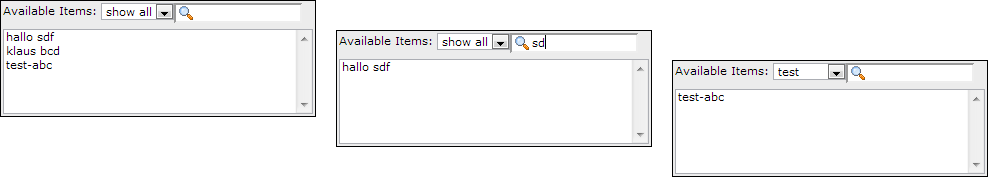
\includegraphics[width=1\linewidth]{Images/InDepthChanges/MultipleValueSelector.png}
	\end{figure}

\end{frame}

% ------------------------------------------------------------------------------
% Improved caching framework by introducing cache groups
% (slide added in March 2014)
% ------------------------------------------------------------------------------
% http://forge.typo3.org/issues/54991

\begin{frame}[fragile]
	\frametitle{Cambios en Profundidad}
	\framesubtitle{Grupos de Caché (1)}

	\begin{itemize}
		\item El núcleo de TYPO3 emplea dos tipos de cachés:

			\begin{itemize}
				\item \textbf{cachés relacionadas con el sistema}:
				caché de carga de clase, caché de configuración, l10n\_cache, extbase\_object, extbase\_reflection etc.
				\item \textbf{cachés relacionadas con el frontend}:
				caché cHash, caché de página, caché de sección de página
			\end{itemize}

		\item En TYPO3 < 6.2, \textit{limpiar todas las cachés} vacía \underline{todas} las cachés, lo que no es ideal

		\item En TYPO3 >= 6.2, el núcleo usa dos grupos de caché:\newline
			"\textbf{páginas}" con todas las cachés relacionadas con la página y "\textbf{sistema}", que es usada para las cachés de tiempo de compilación y configuración

	\end{itemize}

	\begin{figure}
		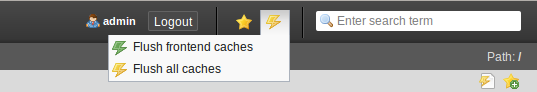
\includegraphics[width=0.5\linewidth]{Images/InDepthChanges/CacheGroups.png}
	\end{figure}

\end{frame}

% ------------------------------------------------------------------------------
% Improved caching framework by introducing cache groups
% (slide added in March 2014)
% ------------------------------------------------------------------------------
% http://forge.typo3.org/issues/54991

\begin{frame}[fragile]
	\frametitle{Cambios en Profundidad}
	\framesubtitle{Grupos de Caché (2)}

	\lstset{
		basicstyle=\tiny\ttfamily
	}

	\begin{itemize}

		\item Opción de configuración relevante:\newline
			\smaller(en ficheros: \texttt{LocalConfiguration.php}/\texttt{DefaultConfiguration.php})\normalsize

			\begin{lstlisting}
			'cache_hash' => array(
			  'frontend' => 'TYPO3\CMS\Core\Cache\Frontend\VariableFrontend',
			  'backend' => 'TYPO3\CMS\Core\Cache\Backend\Typo3DatabaseBackend',
			  'options' => array(),
			  'groups' => array('pages', 'all')
			),
			\end{lstlisting}

		\item El comando "\textit{Vaciar todas las caches}" no vacía más las cachés relacionadas con el sistema
			(sólo "Limpiar la Caché de Configuración" o la Herramienta de Instalación vacía estas cachés)
		\item Una nueva opción userTSconfig habilita a los no administradores para limpiar las cachés de sistema:\newline
			\smaller\texttt{options.clearCache.system = 1}\normalsize

		\breakingchange

	\end{itemize}

\end{frame}

% ------------------------------------------------------------------------------
% TCA: limit number of ticked checkboxes
% (slide added in March 2014)
% ------------------------------------------------------------------------------
% http://forge.typo3.org/issues/55187
% http://forge.typo3.org/issues/55188 (documentation: TCA reference)

\begin{frame}[fragile]
	\frametitle{Cambios en Profundidad}
	\framesubtitle{TCA: Número de Checkboxes Seleccionados}

	\lstset{
		basicstyle=\tiny\ttfamily
	}

	\begin{itemize}
		\item TCA permite la validación del número de checkboxes seleccionados

			\begin{itemize}
				\item \texttt{maximumRecordsChecked}:\newline
					número límite de registros a nivel de sistema
				\item \texttt{maximumRecordsCheckedInPid}:\newline
					número límite de registros a nivel de PID (ID padre)
			\end{itemize}

		\item Si un usuario BE excede el número máximo, el chequeo adicional se revierte hasta que otro registro es deschequeado

		\item Ejemplo:

			\begin{lstlisting}
				$tcaConfiguration = array(
				  'type' => 'check',
				  'eval' => 'maximumRecordsChecked',
				  'validation' => array(
				    'maximumRecordsChecked' => 5
				  )
				);
			\end{lstlisting}

	\end{itemize}

\end{frame}

% ------------------------------------------------------------------------------
% TCA: Introduce MM_oppositeUsage property
% (slide added in March 2014)
% ------------------------------------------------------------------------------
% http://forge.typo3.org/issues/56061
% http://forge.typo3.org/issues/56123 (documentation: TCA reference)

\begin{frame}[fragile]
	\frametitle{Cambios en Profundidad}
	\framesubtitle{TCA: Propiedad \texttt{MM\_oppositeUsage}}

	\lstset{
		basicstyle=\tiny\ttfamily
	}

	\begin{itemize}
		\item Al copiar un registro \texttt{sys\_category}, se crea una nueva referencia MM, pero sin configurar el "fieldname"
		\item Este valor se define básicamente a través de la entidad opuesta con \texttt{MM\_match\_fields}, pero no puede accederse a él
		\item Para manejar este problema, ha sido introducida una nueva propiedad \texttt{MM\_oppositeUsage} para el TCA:

			\begin{lstlisting}
				'config' => array(
				  'allowed' => '*',
				  'MM' => 'tx_myextension_first_second_mm',
				  'MM_oppositeUsage' => array(
				    'tt_content' => array('somefield'),
				    'tx_myextension_domain_model' => array('some_property'),
				  ),
				),
			\end{lstlisting}

	\end{itemize}

\end{frame}

% ------------------------------------------------------------------------------
% Miscellaneous
% ------------------------------------------------------------------------------
% http://forge.typo3.org/issues/49037 (Custom record list in element browser)
% http://forge.typo3.org/issues/36505 (Increase size of be_groups.subgroup field)
% http://forge.typo3.org/issues/49270 (Merge extensions TS/Template)

\begin{frame}[fragile]
	\frametitle{Cambios en Profundidad}
	\framesubtitle{Varios (1)}

	\begin{itemize}

		\item \textbf{Lista de registro personalizado:}\newline
			\small
				Una instancia de la lista de registro personalizado puede ser utilizada en el elemento navegador para reemplazar la lista de registros predeterminada del elemento navegador
			\normalsize

		\item \textbf{Más subgrupos:}\newline
			\small
				El atributo \texttt{subgroup} en la tabla de la Base de Datos \texttt{be\_groups} cambió de \texttt{varchar(250)} a \texttt{text}, lo que permite muchos más subgrupos (usuarios y grupos del backend)
			\normalsize
	\end{itemize}

\end{frame}

% ------------------------------------------------------------------------------
% Miscellaneous
% ------------------------------------------------------------------------------
% http://forge.typo3.org/issues/49037 (Custom record list in element browser)
% http://forge.typo3.org/issues/36505 (Increase size of be_groups.subgroup field)
% http://forge.typo3.org/issues/49270 (Merge extensions TS/Template)

\begin{frame}[fragile]
	\frametitle{Cambios en Profundidad}
	\framesubtitle{Varios (2)}

	\begin{itemize}

		\item \textbf{Extensiones TS/Template fusionadas:}\newline
			\small
				Técnicamente, "WEB > Template" se extendió entre varias extensiones (tstemplate\_ceditor, tstemplate\_info,
tstemplate\_objbrowser and tstemplate\_analyzer). Estas extensiones ahora se combinan en una sola extensión: "tstemplate"
			\normalsize

	\end{itemize}

\end{frame}

% ------------------------------------------------------------------------------
% Miscellaneous
% ------------------------------------------------------------------------------
% http://forge.typo3.org/issues/49721 (Add label_userFunc_options support to BackendUtility)
% http://forge.typo3.org/issues/50441 (Add a timestamp when downloading an extension)
% http://forge.typo3.org/issues/51352 (Force saltedpasswords for Backend)

\begin{frame}[fragile]
	\frametitle{Cambios en Profundidad}
	\framesubtitle{Varios (3)}

	\begin{itemize}

		\item \textbf{label\_userFunc\_option:}\newline
			\small
				Soporte de \texttt{label\_userFunc\_options} añadido a \texttt{BackendUtility}
			\normalsize

		\item \textbf{Nombre del archivo de extensión:}\newline
			\small
				Cuando se descarga una extensión en el Administrador de Extensiones, el nombre de fichero  contiene una marca de tiempo (año, mes, día y hora):\newline
				\texttt{<extensionKey>\_<version>\_<timestamp>.zip}\newline
				\texttt{myextension\_1.0.0\_201312102359.zip}
			\normalsize

		\item \textbf{EXT:saltedpasswords:}\newline
			\small
				Extensión EXT:saltedpasswords es una extensión requerida del sistema y ahora activada por defecto.
				Esto obliga a hashes salted para la autenticación del backend. La Herramienta de Instalación comprueba la configuración y la adapta si es necesario.
			\normalsize

	\end{itemize}

\end{frame}

% ------------------------------------------------------------------------------
% Miscellaneous
% ------------------------------------------------------------------------------
% http://forge.typo3.org/issues/51138 (Allow SignalSlots to modify arguments)
% http://forge.typo3.org/issues/31996 (Transfer query parameters in preview)

\begin{frame}[fragile]
	\frametitle{Cambios en Profundidad}
	\framesubtitle{Varios (4)}

	\begin{itemize}

		\item \textbf{SignalSlots para modificar argumentos:}\newline
			\small
				Los argumentos pasados a SignalSlots dispatcher se pueden modificar ahora y el dispatcher devuelve los argumentos (modificados) tal como los recibió para mantener intacto el encadenamiento.
			\normalsize

		\item \textbf{Previsualización del Espacio de Trabajo:}\newline
			\small
				Ahora se pasan los parámetros de cadena de consulta a la previsualización del espacio de trabajo. Esto era un problema en TYPO3 < 6.2, donde las extensiones a las que se le pasan parámetros personalizados no funcionan correctamente.
			\normalsize

		\item \textbf{Característica PlaceHolder TCEforms:}\newline
			\small
				Introducida en TYPO3 CMS 4.7, la característica PlaceHolder de TCEforms trabaja recursivamente ahora (p.ej. \texttt{\_\_row|uid\_foreign|field}).
			\normalsize
	\end{itemize}

\end{frame}

% ------------------------------------------------------------------------------
% Miscellaneous
% ------------------------------------------------------------------------------
% http://forge.typo3.org/issues/14730 (Support for proxy NTLM authentication)
% http://forge.typo3.org/issues/49667 (Enable double-resolution icons in SpriteGenerator)

\begin{frame}[fragile]
	\frametitle{Cambios en Profundidad}
	\framesubtitle{Varios (5)}

	\begin{itemize}

		\item \textbf{Iconos con resolución doble:}\newline
			\small
				SpriteManager soporta iconos de alta resolución ahora: genera un segundo sprite con iconos de tamaños dobles (un segundo archivo con el sufijo "@x2.png"). CSS3 asegura, que se carga el archivo de alta resolución en dispositivos compatibles\newline
				(esto no afecta al rendimiento en otros dispositivos).
			\normalsize

		\item \textbf{Autenticación proxy NTLM:}\newline
			\small
				Soporte para la autenticación proxy NTLM (\textbf{NT} \textbf{L}AN \textbf{M}anager: un conjunto de protocolos de seguridad de Microsoft) añadido. Esta característica se puede activar en la Herramienta de Instalación:\newline
			\normalsize
			\smaller
				\texttt{\$GLOBALS['TYPO3\_CONF\_VARS']['SYS']['curlProxyNTLM']}\newline
				\emph{(por cierto: esta característica fue solicitada hace más de 8 años :-)}
			\normalsize

	\end{itemize}

\end{frame}

% ------------------------------------------------------------------------------
% Miscellaneous
% (slide added in March 2014)
% ------------------------------------------------------------------------------
% http://forge.typo3.org/issues/14730 (Support for proxy NTLM authentication)

\begin{frame}[fragile]
	\frametitle{Cambios en Profundidad}
	\framesubtitle{Varios (6)}

	\begin{itemize}

		\item \textbf{cookieHttpOnly por defecto:}\newline
			\small
				Para hacer que la cookie de sesión sea sólo accesible a través del protocolo HTTP, ahora se activa \texttt{cookieHttpOnly} por defecto.\newline
				Esto significa que las cookies "fe\_typo\_user" y "be\_typo\_user" no estarán accesibles para lenguajes de scripting (p.ej. JavaScript), lo que endurece la protección contra ataques XSS (\textit{cross site scripting}). Sin embargo, algunos navegadores antiguos no soportan esta técnica.
			\normalsize

		\item \textbf{Limpiar Tabla de Base de Datos:}\newline
			\small
				Los siguientes atributos se han eliminado de la tabla de DB \texttt{tt\_content} (no usados desde TYPO3 4.0):
				\texttt{text\_align}, \texttt{text\_face}, \texttt{text\_size}, \texttt{text\_color}, \texttt{text\_properties}.
			\normalsize

	\end{itemize}

\end{frame}

% ------------------------------------------------------------------------------
% Miscellaneous
% (slide added in March 2014)
% ------------------------------------------------------------------------------
% https://forge.typo3.org/issues/55190 (Move Tidy functionality to a TER extension)

\begin{frame}[fragile]
	\frametitle{Cambios en Profundidad}
	\framesubtitle{Varios (7)}

	\begin{itemize}

		\item \textbf{Eliminada HTML Tidy:}\newline
			\small
				La funcionalidad \textit{HTML Tidy} ha sido eliminada del núcleo TYPO3. Puede ser fácilmente restaurada installando EXT:tidy del TER.
			\normalsize

		\item \textbf{Eliminada dontSetCookie:}\newline
			\small
				Debido al hecho de que la cookie "fe\_typo\_user" sólo se configura si se requiere (y no siempre), la opción \texttt{dontSetCookie} de la Herramienta de Instalación se convirtió en irrelevante y ha sido eliminada.
			\normalsize

		\item \textbf{Eliminados los scripts "Wizard":}\newline
			\small
				Eliminación de los siguiente scripts "wizard":
				\texttt{typo3/wizard\_add.php}, \texttt{typo3/wizard\_colorpicker.php}, \texttt{typo3/wizard\_edit.php}, \texttt{typo3/wizard\_forms.php}, \texttt{typo3/wizard\_list.php}, \texttt{typo3/wizard\_rte.php}, \texttt{typo3/wizard\_table.php}
			\normalsize

	\end{itemize}

\end{frame}

% ------------------------------------------------------------------------------

